\documentclass[letter]{article}
\renewcommand{\baselinestretch}{1.25}

\usepackage[margin=1in]{geometry}
\usepackage{physics}
\usepackage{amsmath, amsfonts, amssymb, amsthm}
\usepackage{amssymb}
\numberwithin{equation}{section}
\usepackage{amssymb}
\usepackage{graphicx}
\usepackage{hyperref}
\usepackage{empheq}
\usepackage{pdfpages}

% Math Proof things
\newcommand{\Rel}{\mathcal{R}}
\newcommand{\R}{\mathbb{R}}
\newcommand{\C}{\mathbb{C}}
\newcommand{\N}{\mathbb{N}}
\newcommand{\Z}{\mathbb{Z}}
\newcommand{\Q}{\mathbb{Q}}

\newcommand{\st}{\ : \ }

% Theorem Definition
\newtheorem{definition}{Definition}
\newtheorem{assumption}{Assumption}
\newtheorem{theorem}{Theorem}
\newtheorem{lemma}{Lemma}
\newtheorem{proposition}{Proposition}
\newtheorem{example}{Example}


% % MATLAB Formatting Code
% \usepackage[numbered,framed]{matlab-prettifier}
% \lstset{style=Matlab-editor,columns=fullflexible}
% \renewcommand{\lstlistingname}{Script}
% \newcommand{\scriptname}{\lstlistingname}

\allowdisplaybreaks

%opening
\title{MECH 6323 - HW 3}
\author{Jonas Wagner}
\date{2022, March 1\textsuperscript{st}}

\begin{document}	

\maketitle

\tableofcontents

%----- Problem 1 -----------------------------------------------------------------------
\newpage
\section{Problem 1}
\subsection*{Preliminaries:}
\begin{definition}
    \textbf{Matrix Basics:} 
    For $A \in \C^{n \cross m}$ and $x \in \C^{m}$,
    \begin{enumerate}
        \item The \emph{\underline{Eigenvalues}} ($\lambda_i$) and \emph{\underline{Eigenvectors}} ($x_i$) of $A$ are defined as the solutions to \[
            \lambda_i A = \lambda_i x_i
        \] \item The \emph{\underline{Spectral Radius}} of $A$ is defined as \[
            \rho(A) := \max_{i} \abs{\lambda_i(A)}
        \]
    \end{enumerate}
\end{definition}

\begin{definition}
    \textbf{Vector Norms:} 
    For $x \in \C^{n}$,
    \begin{enumerate}
        \item The \emph{\underline{$2$-norm}}, or \emph{\underline{Euclidean norm}}, is defined as\[
            \norm{x}_2 := \sqrt{\sum_{i=1}^{n} x_{i}^{2}}
        \] \item The \emph{\underline{$1$-norm}} is defined as\[
            \norm{x}_1 := \sum_{i=1}^{n} \abs{x_{i}}
        \] \item The \emph{\underline{$\infty$-norm}} is defined as\[
            \norm{x}_\infty := \max{i = 1,\dots,n} \abs{x_{i}}
        \] \item The \emph{\underline{p-norm}} is defined as\[
            \norm{x}_p := \qty[\sum_{i=1}^{n} \abs{x_{i}}^{p}]^{\frac{1}{p}}
        \]
    \end{enumerate}
\end{definition}

\begin{definition}
    \textbf{Matrix Norms:}
    For $A \in \C^{n \cross m}$ and $x \in \C^{m}$, \begin{enumerate}
        \item The \emph{\underline{Induced $2$-norm}} is defined as \[
            \norm{A}_{2\to2} := \sup_{x \neq 0} \cfrac{\norm{A x}_2}{\norm{x}_2}
        \] and is also known as the \emph{\underline{spectral norm}} and has the additional properties of \begin{enumerate}
            \item $\norm{A}_{2\to2} = \sqrt{\lambda_{max}(A^* A)} = \overline{\sigma}(A)$
            \item $\norm{A^*A}_{2\to2} = \norm{A A^*}_{2\to2} = \norm{A}_2^2$
        \end{enumerate}
    \end{enumerate}
\end{definition}

%---- 1a
\subsection{}
\subsubsection*{Problem:}
For $M \in \C^{n \cross m}$, show that for all $x \in \C^m$ \[
    \norm{M x}_2 \leq \norm{M}_{2\to 2} \norm{x}_2
\]

\subsubsection*{Solution:}
\begin{theorem}
    For $M \in \C^{n \cross m}$, show that for all $x \in \C^m$ \[
        \norm{M x}_2 \leq \norm{M}_{2\to 2} \norm{x}_2
    \]
    \begin{proof}
        From the definition of the $2$-norm, we have\[
            \norm{M}_{2\to2} := \sup_{x \neq 0} \cfrac{\norm{A x}_2}{\norm{x}_2}
        \]\begin{align*}
            \norm{M}_{2\to2} &= \sup_{x \neq 0} \cfrac{\norm{A x}_2}{\norm{x}_2}\\
            \norm{M}_{2\to2} \norm{x}_2 &= \sup_{x \neq 0} \cfrac{\norm{M x}_2}{\norm{x}_2} \norm{x}_2\\
                &= \sup_{x \neq 0} \norm{M x}_2\\
            \Aboxed{
                \norm{M}_{2\to2} \norm{x}_2 
                    &\geq \norm{M x}_2 \ \forall_{x \in C^{m}}
            }
        \end{align*}
    \end{proof}
\end{theorem}


%---- 1b
\subsection{}
\subsubsection*{Problem:}
Let $\{\lambda_i\}_{i=1}^{n}$ denote the eigenvalues of $A\in \C^{n\cross n}$.
Show that $\rho(A) \leq \norm{A}_{2\to 2}$, where $\rho(A)$ is the spectral radius of matrix $A$.
i.e. $\rho(A) := \max_{i} \abs{\lambda_i(A)}$.

\subsubsection*{Solution:}
\begin{theorem}
    Let $A \in \C^{n\cross n}$.
    The spectral radius $\rho(A)$ will always be smaller then the induced $2$-norm.
    i.e.\[
        \rho(A) \leq \norm{A}_{2\to 2}
    \]
    \begin{proof}
        From the definition of the induced $2$-norm, we have\[
            \norm{M}_{2\to2} := \sup_{x \neq 0} \cfrac{\norm{A x}_2}{\norm{x}_2}
        \] Additionally, from the definition of the vector $2$-norm \[
            \norm{x}_{2}^{2} = x^T x
        \]
        \begin{align*}
            \norm{M}_{2\to2} 
                &= \sup_{x \neq 0} \cfrac{\norm{A x}_2}{\norm{x}_2}\\
            \qty(\norm{M}_{2\to2})^2 
                &= \sup_{x \neq 0} \qty(\cfrac{\norm{A x}_2}{\norm{x}_2})^2\\
                &= \sup_{x \neq 0} \cfrac{(Mx)^T M x}{x^T x}\\
                &= \sup_{x \neq 0} \cfrac{x^T M^T M x}{x^T x}\\
            \intertext{Since $\forall_{x} M x \leq M x_{max}$, where $x_{max}= \norm{x}_2 v_{max}$ and $v_{max}$ is the eigenvector associated with $\lambda_{max} = \rho(A)$}
                &\leq \sup_{x \neq 0} \cfrac{x_{max}^T M^T M x_{max}}{x^T x}\\
                &= \sup_{x \neq 0} \cfrac{\norm{x}_2 v_{max}^T \lambda_{max} \lambda{max} \norm{x}_2 v_{max}}{x^T x}\\
                &= \sup_{x \neq 0} \cfrac{v_{max}^T \norm{x}_2^2 \lambda_{max}^2 v_{max}}{x^T x}\\
                &= \sup_{x \neq 0} \cfrac{\lambda_{max}^2 \norm{x}_2^2 \norm{v_{max}}_2^2}{\norm{x}_2^2}\\
                &= \sup_{x \neq 0} \cfrac{\lambda_{max}^2 \norm{x}_2^2 (1)^2}{\norm{x}_2^2}\\
                &= \sup_{x \neq 0} \lambda_{max}^2\\
                &= \lambda_{max}^2 = \rho(A)^2\\
            \qty(\norm{M}_{2\to2})^2 
                &\leq (\rho(A))^2\\
            \Aboxed{
                \norm{M}_{2\to2} &\leq \rho(A)
            }
        \end{align*}
    \end{proof}
\end{theorem}

%---- 1c
\subsection{}
\subsubsection*{Problem:}
Let $A \in \C^{n\cross m}$ and $B \in \C^{m\cross k}$.
Prove the multiplicative property of the induced 2-norm.\[
    \norm{AB}_{2\to 2} \leq \norm{A}_{2\to 2} \norm{B}_{2\to2}
\].

\subsubsection*{Solution:}
\begin{theorem}
    Let $A \in \C^{n\cross m}$ and $B \in \C^{m\cross k}$.
    Just like in all norms by definition, \[
        \norm{AB}_{2\to 2} \leq \norm{A}_{2\to 2} \norm{B}_{2\to2}
    \]
    \begin{proof}
        From norm definitions,\[
            \norm{A x}_{2} \leq \norm{A}_{2\to 2} \norm{x}_{2}
        \] and therefore $\forall_{x \in \C^{k}}$,\begin{align*}
            \norm{A B x}_{2} 
                &\leq \norm{A}_{2\to 2} \norm{B x}_{2}\\
                &\leq \norm{A}_{2\to 2} \norm{B}_{2\to2} \norm{x}_{2}
            \intertext{
                Taking $x = \sigma \hat{x}$ where magnitude $\sigma = \norm{x}_2$ and $\hat{x}$ is the associated unit vector for $x$.
                Also, $\norm{\sigma \hat{x}} = \sigma \norm{\hat{x}}_2 = \norm{x}_2$
            }
            \norm{A B \norm{x}_2 \hat{x}}_2
                &\leq \norm{A}_{2\to2} \norm{B}_{2\to2} \norm{x}_2 \norm{\hat{x}}_2\\
            \norm{x}_2 \norm{A B \hat{x}}_2 
                &\leq \norm{A}_{2\to2} \norm{B}_{2\to2} \norm{x}_2 (1)\\
            \intertext{
                Noting that $\norm{A B \hat{x}}_2 \leq \norm{A B}_{2\to2} \norm{\hat{x}}_2 = \norm{A B}_{2\to2} \norm{\hat{x}}_2$.
                Thus, $\norm{A B \hat{x}}_2 = \norm{A B}_{2\to 2}$
            }
            \norm{x}_2 \norm{A B}_\norm{2\to2}
                &\leq \norm{A}_{2\to2} \norm{B}_{2\to2} \norm{x}_2\\
            \Aboxed{
                \norm{A B}_\norm{2\to2} 
                    &\leq \norm{A}_{2\to2} \norm{B}_{2\to2}
            }
        \end{align*} 
    \end{proof}
\end{theorem}

%---- 1d
\subsection{}
\subsubsection*{Problem:}
Let $x\in \C^m$ and $y \in \C^n$.
Show that if $\norm{y}_2 \leq \norm{x}_2$, then there exists a $\Delta \in \C^{n\cross m}$ such that $y = \Delta x$ and $\overline{\sigma(\Delta)}\leq 1$.
The choice of $\Delta$ should only be expressed in terms of $x$, $y$, and their norms.
Conversely, show that if $\norm{y}_2 > \norm{x}_2$, then there is no $\Delta \in \C^{n\cross m}$ such that $y = \Delta x$ and $\overline{\sigma(\Delta)}\leq 1$.

\subsubsection*{Solution:}
\begin{theorem}
    Let $x \in \C^m$ and $y \in \C^n$.
    There exists a $\Delta \in \C^{n\cross m}$ such that $y = \Delta x$ and $\overline{\sigma(\Delta)}\leq 1$ if and only if $\norm{y}_2 \leq \norm{x}$.
    i.e.\[
        \exists_{\Delta \in \C^{n\cross m}} \st y = \Delta x \land \overline{\sigma(\Delta)}\leq 1
        \iff \norm{y}_2 \leq \norm{x}_2
    \]
    \begin{proof}
        From $y = \Delta x$ we have \begin{align*}
            y &= \Delta x\\
            y x^* &= \Delta x x^*\\
            \Delta 
                &= \cfrac{y x^*}{x x^*}\\
                &= \cfrac{y x^*}{\norm{x}_2^2}
        \end{align*}
        From the definition of the induced 2-norm,\[
            \overline{\sigma}(\Delta) = \norm{\Delta}_{2\to2} 
                = \sup_{x \neq 0} \cfrac{\norm{\Delta x}_2}{\norm{x}_2}
        \] Then in order for $\overline{\sigma(\Delta)}\leq 1$, \begin{align*}
            1 \geq \overline{\sigma}(\Delta) 
                &= \norm{\Delta}_{2\to2}\\
                &= \sup_{x \neq 0} \cfrac{\norm{\Delta x}_2}{\norm{x}_2}\\
                &= \sup_{x \neq 0} \cfrac{\norm{\cfrac{y x^*}{\norm{x}_2^2} x}_2}{\norm{x}_2}\\
            \qty(1)^2
                &\geq \qty(\sup_{x \neq 0} \cfrac{\norm{\cfrac{y x^*}{\norm{x}_2^2} x}_2}{\norm{x}_2})^2\\
            1   
                &\geq \sup_{x \neq 0} \cfrac{\norm{\cfrac{y x^*}{\norm{x}_2^2}x}_2^2}{\norm{x}_2^2}\\
                &= \sup_{x \neq 0} \cfrac{
                    \qty(\cfrac{y x^*}{\norm{x}_2^2}x)^* \qty(\cfrac{y x^*}{\norm{x}_2^2}x)
                    }{\norm{x}_2^2}\\
                &= \sup_{x \neq 0} \cfrac{x^* \cfrac{x y^* y x^*}{\norm{x}_2^4} x
                    }{\norm{x}_2^2}\\
                &= \sup_{x \neq 0} \cfrac{x^* x y^* y x^* x}{\norm{x}_2^6}\\
                &= \sup_{x \neq 0} \cfrac{\norm{x}_2^2 \norm{y}_2^2 \norm{x}_2^2}{\norm{x}_2^6}\\
                &= \sup_{x \neq 0} \cfrac{\norm{y}_2^2}{\norm{x}_2^2}\\
            \Aboxed{
                1 &\geq \sup_{x \neq 0} \cfrac{\norm{y}_2}{\norm{x}_2}
            }
        \end{align*}
        Clearly this is true if and only if $\norm{y}_2 \leq \norm{x}_2$.
    \end{proof}
\end{theorem}


%----- Problem 2 -----------------------------------------------------------------------
% \newpage
\section{Problem 2}
See attached MATLAB .mlx script.
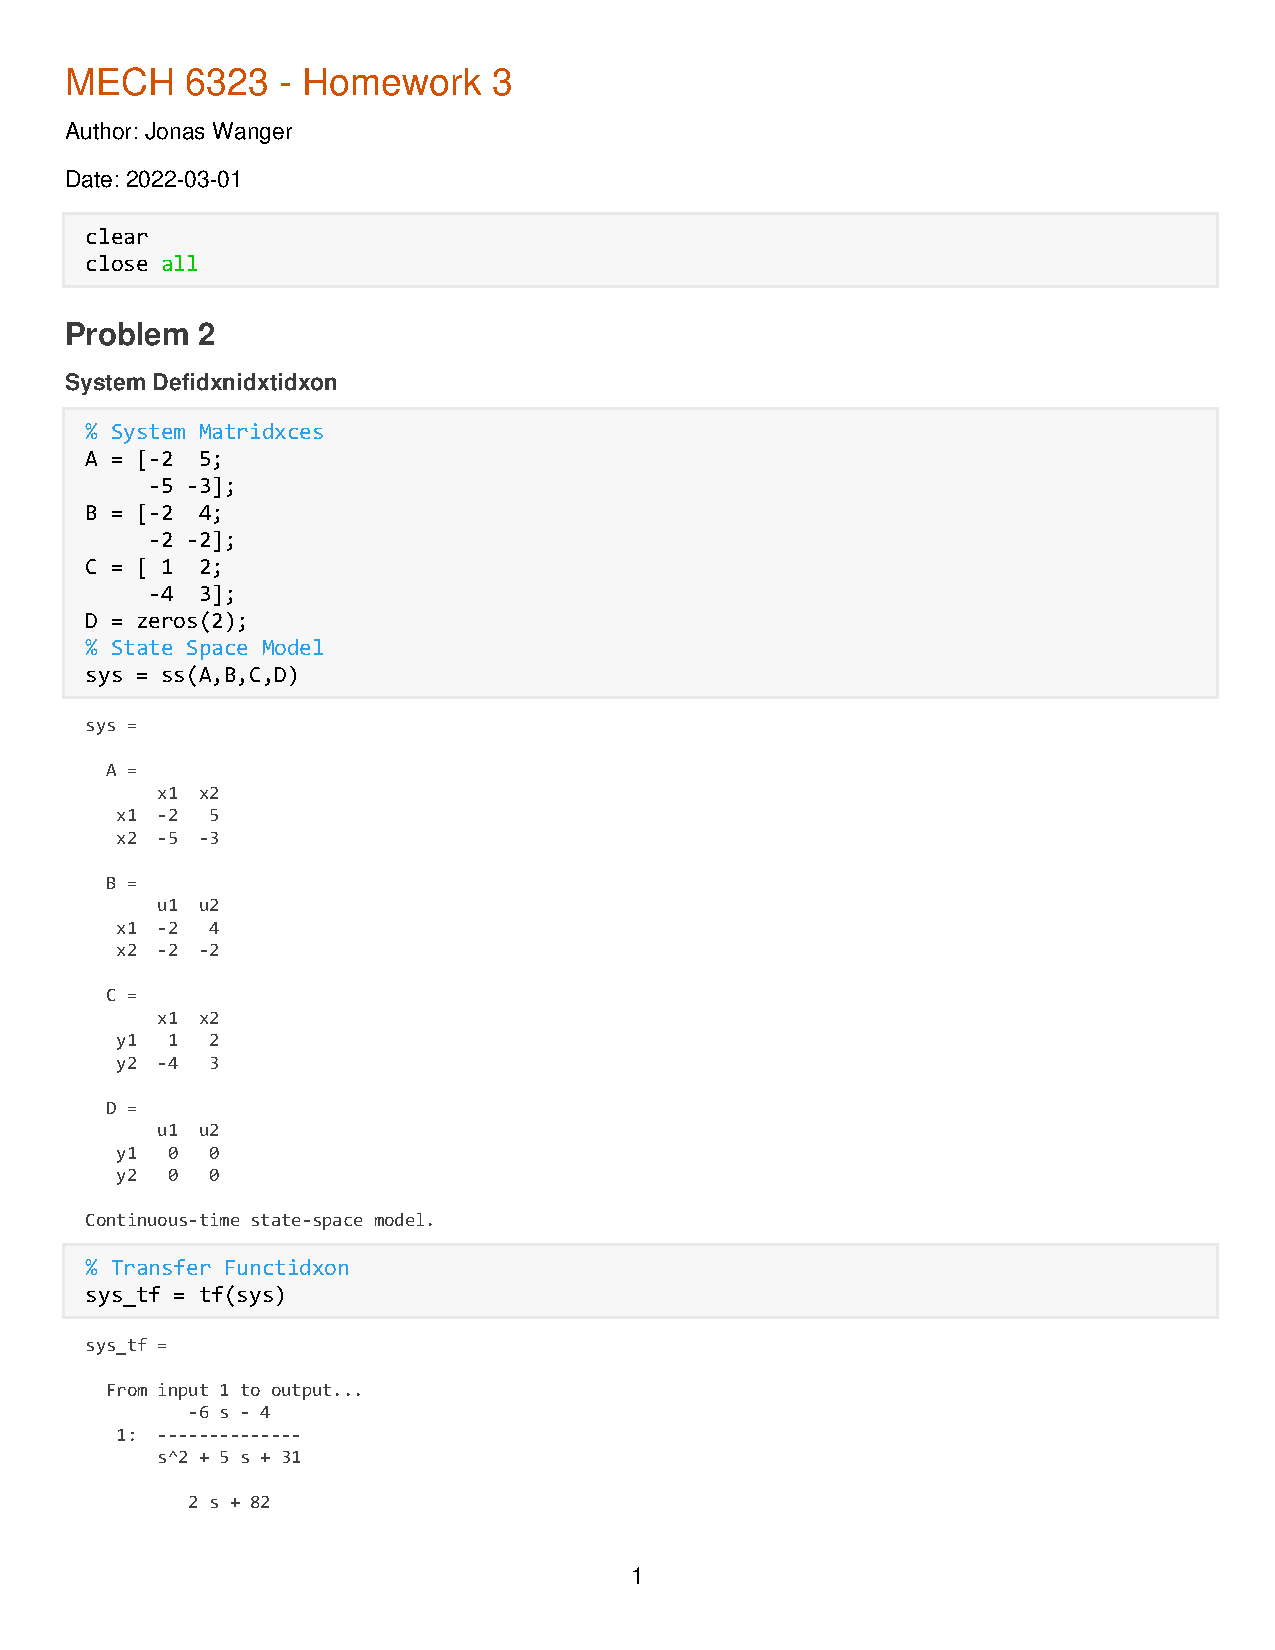
\includepdf[pages=-]{MECH6323_HW03.pdf}

%----- Problem 3 -----------------------------------------------------------------------
\newpage
\section{Problem 3}
\subsubsection*{Problem:}
Let $S$ and $T$ denote the sensitivity and complementary sensitivity closed-loop transfer functions.
Prove that\[
    \norm{S}_\infty \geq \norm{T}_\infty - 1
\]
\subsubsection*{Preliminaries}
\begin{definition}
    Let $P$ and $C$ represent the plant and controller transfer functions respectively. 
    Within a standard unity feedback system, \begin{enumerate}
        \item the \underline{\emph{sensitivity closed-loop transfer function}} is defined as:\[
            S = \cfrac{1}{1+PC}
        \] \item the \underline{\emph{complementary sensitivity closed-loop transfer function}} is defined as:\[
            T = \cfrac{PC}{1+PC}
        \]
    \end{enumerate}
\end{definition}
\subsubsection*{Solution:}
\begin{theorem}
    Let $P$ and $C$ represent the plant and controller transfer functions respectively. 
    Within a standard unity feedback system, \[
        \norm{S}_\infty \geq \norm{T}_\infty - 1
    \]
    \begin{proof}
        From the definitions, \[
            T - S = \cfrac{PC}{1+PC} - \cfrac{1}{1+PC} = \cfrac{-1 + PC}{1 + PC}
        \] Applying the $\infty-$norm,\[
            \norm{T - s}_\infty = \norm{\cfrac{-1 + PC}{1 + PC}}_infty
        \] Since ${-1 + PC} < {1 + PC}$, \[
            \norm{T - S}_\infty \leq 1
        \] From the triangular inequality we have\[
            \norm{T - S}_\infty \geq \norm{T}_\infty - \norm{S}_\infty
        \] And thus,\[\boxed{
            1 \geq \norm{T - S}_\infty \geq \norm{T}_\infty - \norm{S}_\infty
            \implies \norm{S}_\infty \geq \norm{T}_\infty - 1
        }\]
    \end{proof}
\end{theorem}

\newpage
\appendix
\section{MATLAB Code:}\label{apx:matlab}
See attached.
Additionally, all the code I write in this course can be found on my GitHub repository:\\
\href{https://github.com/jonaswagner2826/MECH6323}{https://github.com/jonaswagner2826/MECH6323}






\end{document}
